\documentclass[10pt]{article}
\usepackage[margin=17mm]{geometry}
\usepackage{graphicx,booktabs,hyperref}
\usepackage[strings]{underscore}
\setlength{\parindent}{0pt}\setlength{\parskip}{4pt}
\begin{document}
\section*{X-only fixtures: declared-subgroup audit v2}
Native relevance check, 2026-10-25, source 5b36e4945d3b. All seven original and
1,152 fresh targets are retained. Each x is checked on E0 ($a=0,b=1$) and a
trace-one-a quadratic twist in its exact field, with the largest odd prime r
and an explicitly verified generator G. These choices qualify the fixtures;
they do not retrofit a curve, subgroup or query law into the original input.

\begin{center}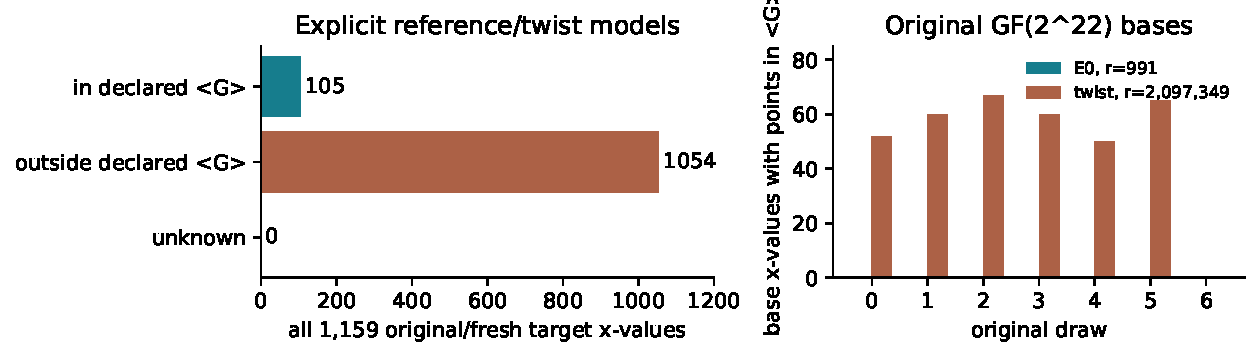
\includegraphics[width=\linewidth]{subgroup-status.pdf}\end{center}
Coprime r/cofactor proves uniqueness. For the remaining GF($2^{10}$), r=11 model, complete enumeration of the actual 11-point subgroup resolves all 152 earlier nulls. The first receipt is unchanged.

\begin{center}\begin{tabular}{rrrrrr}\toprule
Draw & Boolean roots & E0 target in G & twist target in G & E0 base x & twist base x\\\midrule
0 & 0 & no & no lift & 0 & 52 \\
1 & 6 & no & no lift & 0 & 60 \\
2 & 6 & no & no lift & 0 & 67 \\
3 & 0 & no & no lift & 0 & 60 \\
4 & 18 & no lift & yes & 0 & 50 \\
5 & 0 & no lift & no & 0 & 65 \\
6 & 0 & no & no lift & 0 & 0 \\
\bottomrule\end{tabular}\end{center}
The original field is GF($2^{22}$), modulus $z^{22}+z+1$.
E0 has order $991\cdot4232$; the chosen twist has a=$2^{21}$, order
$2\cdot2,097,349$. Base columns count distinct abscissae supporting points
in the indicated subgroup. Original draw 6 has none on either model; its
zero-guess refutation remains finite Boolean evidence, not a verified
ordinary subgroup-query result.

All three deterministically selected original SAT witnesses give two
signed curve relations on their matching model, after testing all eight
signed tuples. The amended audit explicitly finds zero usable-subgroup relations for each selected witness; at least one summand is outside the declared subgroup. This checks one witness per SAT draw, not every
solution; fresh SAT witnesses are not tested by this run.

Orders use the exact E0/F2 Frobenius recurrence and complementary twist
order, controlled by exhaustive small-field point counts. Full exact
factorizations and deterministic u64 primality checks bind r. Every target
root passes substitution, an independent trace criterion, library point
membership and full-order annihilation. G is nonidentity and [r]G=O.
The repeated-prime control rejects r-torsion outside the actual G subgroup.
The native JSON binds all models, unregistered EC1 record identities,
generators and 37 input hashes. A fresh native rerun is byte-identical.

Scope: model-specific finite membership, not an ordinary query distribution,
general curve validity, closure-degree law, full relation enumeration,
complete DLP price or speedup. Local shared x86-64 host, L0; 12-GiB
address-space and 900-second limits, exit 0. No paid allocation.
Protocol: SUBGROUP_RELEVANCE_PROTOCOL.md; amendment: SUBGROUP_RELEVANCE_AMENDMENT.md.
Receipt: \path{../../pipeline-receipts/fixture-subgroups-enumerated-20261025/receipt.json}.
\end{document}
